% !TeX program = xelatex
\documentclass[a4paper, 8pt]{extarticle}
\usepackage[total={210mm, 279.4mm}, width=170mm, top=20mm, left=20mm, right=20mm, bottom=20mm]{geometry}
\newcommand{\template}[1]{}

\newlength{\headerColumn}
\setlength{\headerColumn}{2.5cm}
\newlength{\firstColumn}
\setlength{\firstColumn}{2cm}
\newlength{\lastColumn}
\setlength{\lastColumn}{6cm}

%A Few Useful Packages
\usepackage[german, english]{babel}
\selectlanguage{german}
\usepackage{calc}
\usepackage{tabularx}
\usepackage[document]{ragged2e}
\usepackage{lipsum}
\usepackage{multirow}
\usepackage{marvosym}
\usepackage{fontspec} 					%for loading fonts
\usepackage{xunicode, xltxtra, url, parskip} 	%other packages for formatting
\RequirePackage{color, graphicx}
\usepackage[usenames, dvipsnames]{xcolor}
%\usepackage[big]{layaureo} 				%better formatting of the A4 page
% an alternative to Layaureo can be ** \usepackage{fullpage} **
\usepackage{supertabular} 				%for Grades
\usepackage{titlesec}					%custom \section
\usepackage{colortbl}
\usepackage{xcolor}

%Setup hyperref package, and colours for links
\usepackage{hyperref}
\definecolor{linkcolor}{rgb}{0, 0.0, 0.0}
\hypersetup{colorlinks, breaklinks, urlcolor=linkcolor, linkcolor=linkcolor, filecolor=linkcolor, linkbordercolor=linkcolor, urlbordercolor=linkcolor, filebordercolor=linkcolor}
\makeatletter
\Hy@AtBeginDocument{%
	\def\@pdfborder{0 0 0}% Overrides border definition set with colorlinks=true
	\def\@pdfborderstyle{/S/U/W 0.5}% Overrides border style set with colorlinks=true
	% Hyperlink border style will be underline of width 1pt
}
\makeatother

%FONTS
\hyphenchar\font=-1
\hyphenpenalty=1000
\exhyphenpenalty=1000
\defaultfontfeatures{Mapping=tex-text}
\linespread{1.3}
%\setmainfont[SmallCapsFont = Fontin SmallCaps]{Fontin}
%%% modified for Karol Kozioł for ShareLaTeX use
%\setmainfont[
%SmallCapsFont = Fontin-SmallCaps.otf,
%BoldFont = Fontin-Bold.otf,
%ItalicFont = Fontin-Italic.otf
%]
%{Fontin.otf}
%%%
\setmainfont[
BoldFont = cmunrb.otf,
ItalicFont = cmunsl.otf,
BoldItalicFont = cmunbl.otf
]{cmunrm.otf}

%CV Sections inspired by:
%http://stefano.italians.nl/archives/26
\titleformat{\section}{\Large\bfseries\raggedright}{}{0em}{}[\titlerule]
\titlespacing{\section}{0pt}{3pt}{3pt}
%Tweak a bit the top margin
%\addtolength{\voffset}{-1.3cm}

%-------------WATERMARK TEST [**not part of a CV**]---------------
\usepackage[absolute]{textpos}
%\usepackage{fancyhdr}

\setlength{\TPHorizModule}{30mm}
\setlength{\TPVertModule}{\TPHorizModule}
\textblockorigin{2mm}{0.65\paperheight}
\setlength{\parindent}{0pt}
\setlength{\parskip}{1em}
\newlength\savedwidth
\definecolor{hbar}{HTML}{808080}
\newcommand\whline[1]{\arrayrulecolor{hbar}\noalign{\global\savedwidth\arrayrulewidth\global\arrayrulewidth 2pt}%
\cline{#1}
\noalign{\global\arrayrulewidth\savedwidth}}
%\renewcommand{\textbf}[1]{\scalebox{0.8}[1]{\bfseries #1}}
\usepackage{scrpage2}
\pagestyle{scrheadings} % non-numbered pages

\ihead[]{}
\chead[]{}
\ohead[]{}
\ifoot[]{}
\cfoot[Leonhard  Euler]{Leonhard  Euler}
\ofoot[\pagemark]{\pagemark}
%--------------------BEGIN DOCUMENT----------------------
\begin{document}
\hyphenation{Bachelor-arbeit Master-arbeit Programmier-sprachen Frei-willigen-arbeit Doktor-arbeit}
%WATERMARK TEST [**not part of a CV**]---------------
%\font\wm=''Baskerville:color=787878'' at 8pt
%\font\wmweb=''Baskerville:color=FF1493'' at 8pt
%{\wm
%	\begin{textblock}{1}(0, 0)
%		\rotatebox{-90}{\parbox{500mm}{
%			Typeset by Alessandro Plasmati with \XeTeX\  \today\ for
%			{\wmweb \href{http://www.aleplasmati.comuv.com}{aleplasmati.comuv.com}}
%		}
%	}
%	\end{textblock}
%}



\font\fb=''[cmr10]'' %for use with \LaTeX command

%--------------------TITLE-------------
\par{\Huge \bfseries \scalebox{1.2}[1.2]{Curriculum Vitae [Leonhard  Euler]}
\bigskip\par}

%--------------------SECTIONS-----------------------------------
%Section: Personal Data

\begin{tabular}{p{\headerColumn}p{2.6cm}p{21mm}p{\textwidth-\headerColumn-2.6cm-21mm-16mm}}
	\whline{2-4}\\
[0.1mm]
	\multirow[t]{7}{\headerColumn}{\Large\bfseries\raggedleft Persönliche Informationen}
	&
	\multirow{7}{2.6cm}{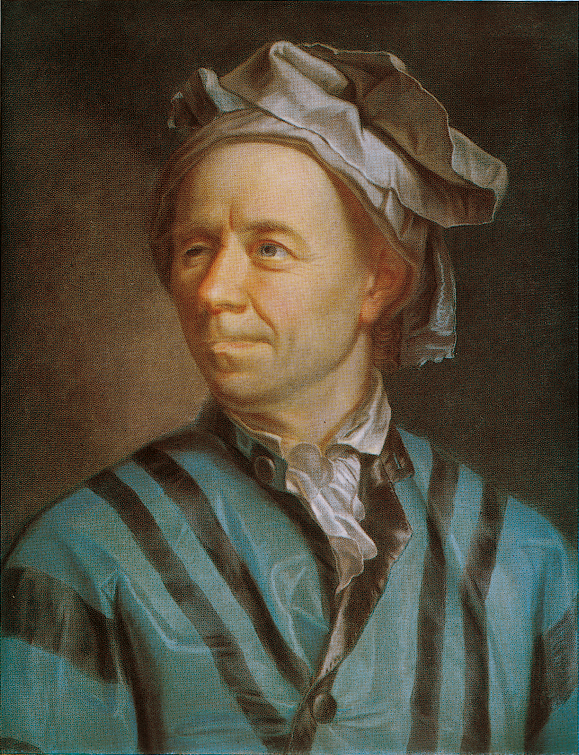
\includegraphics[width=2.6cm, height=3.466cm]{img/mypics/Leonhard_Euler_by_Handmann.png}}
	&
	 \raggedleft Geburtsdatum:& \textbf{15. April 1707} \\
	 &&\raggedleft Nationalität:&  \textbf{Schweiz}\\
	 &&\raggedleft Adresse:& \textbf{Baselstrasse 32, 4125 Riehen, Schweiz} \\
	 &&\raggedleft Email:& \textbf{\href{l.euler@swissmail.com}{l.euler@swissmail.com}}\\
	 &&\raggedleft Telefonnummer:& \textbf{+41 53 669 25 91}\\
	 &&\raggedleft Github:& \textbf{\href{https://github.com/leuler}{https://github.com/leuler}}\\
	 &&\raggedleft LinkedIn:& \textbf{\href{https://linkedin.com/in/leuler}{https://linkedin.com/in/leuler}}\\
[5mm]
\end{tabular}
\vskip 0mm
\begin{tabular}{p{\headerColumn}p{\textwidth-\headerColumn-8mm}}
	\whline{2-2}&\\
	\Large\bfseries\raggedleft Vorstellung&
	\par{Ich bin einer der bedeutedsten Mathematiker der Geschichte und lieferte Beiträge in unterschiedlichen Teilgebieten wie: Mathematische Notation, Analysis, Kombinatorik, Graphentheorie, Phsyik und Musiktheorie.}
\end{tabular}
%\extrarowheight=0.15cm
\vskip 0mm
%Section: Works
\begin{tabular}[t]{p{\headerColumn}p{\textwidth-\headerColumn-8mm}}
	\whline{2-2}&\\
	\Large\bfseries\raggedleft Arbeiten&
\begin{tabular}[t]{p{\firstColumn}p{\textwidth-\firstColumn-\headerColumn-16mm}}
	
	\multirow[t]{3}{\firstColumn}{ \raggedleft \large\textbf{Doktorarbeit}} & \textbf{De Sono}\\
		&\par{\textbf{Supervisoren:}
		\href{https://en.wikipedia.org/wiki/List_of_placeholder_names_by_language}{Prof. M. Mustermann}, B. Name }\\
		&\par{\textit{Ich beschreibe mathematische modelle welche die Ausbreitung von Schallwellen abbilden.}}\\
		&\par{\textbf{Tech-Stack}:
		Python, Phsysics Simulations, Mathematics, Git }\\
\end{tabular}
\end{tabular}

%Section: Education
\begin{tabular}[t]{p{\headerColumn}p{\textwidth-\headerColumn-8mm}}
	\whline{2-2}&\\
	\Large\bfseries\raggedleft Ausbildung&
\begin{tabular}[t]{p{\firstColumn}p{\textwidth-\lastColumn-\firstColumn-\headerColumn-16mm}p{\lastColumn}}
\raggedleft 1720 - 1723 & \textbf{Master in Philosophie} & \href{https://unibas.ch/}{Universität Basel [UniBas]}\\
\raggedleft 1725 - 1726 & \textbf{Ph.D. in Physik} & \href{https://unibas.ch/}{Universität Basel [UniBas]}\\
\end{tabular}
\end{tabular}

%Section: Work Experience
\begin{tabular}[t]{p{\headerColumn}p{\textwidth-\headerColumn-8mm}}
	\whline{2-2}&\\
	\Large\bfseries\raggedleft Erfahrung&
\begin{tabular}[t]{p{\firstColumn}p{\textwidth-\firstColumn-\lastColumn-\headerColumn-16mm}p{\lastColumn}}
	\raggedleft 1741 - 1766 & \textbf{Mathematiker} & \href{https://de.wikipedia.org/wiki/K%C3%B6niglich_Preu%C3%9Fische_Akademie_der_Wissenschaften_zu_Berlin}{Königlich Preußischen Akademie der Wissenschaften zu Berlin}\\
		&\multicolumn{2}{p{\textwidth-\firstColumn-\headerColumn-16mm}}{\par{\textit{Ich arbeitete an unterschiedlichen Problemen in der Mathematik}}}\\
		&\multicolumn{2}{p{\textwidth-\firstColumn-\headerColumn-16mm}}{\par{\textbf{Tech-Stack:}
		Mathematics, Python, Docker, Latex, Git 
		}}\\
\raggedleft 1727 - 1741 & \textbf{Mathematiker} & \href{https://de.wikipedia.org/wiki/Sankt_Petersburg}{Kaiserlich Russische Akademie der Wissenschaften in Sankt Petersburg}\\
		&\multicolumn{2}{p{\textwidth-\firstColumn-\headerColumn-16mm}}{\par{\textit{Ich arbeitete an unterschiedlichen Problemen in der Mathematik}}}\\
		&\multicolumn{2}{p{\textwidth-\firstColumn-\headerColumn-16mm}}{\par{\textbf{Tech-Stack:}
		Mathematics, Python, Docker, Latex, Git 
		}}\\
\end{tabular}
\end{tabular}

\begin{tabular}[t]{p{\headerColumn}p{\textwidth-\headerColumn-8mm}}
	\whline{2-2}&\\
	\Large\bfseries\raggedleft Fähigkeiten&
\begin{tabular}[t]{p{\firstColumn}p{\textwidth-\firstColumn-\lastColumn-\headerColumn-16mm}p{\lastColumn}}
	\multirow[t]{2}{\firstColumn}{\raggedleft \textbf{Sprachen}}
	 & \raggedleft
	Deutsch 
	& Muttersprache\\
	& \raggedleft Englisch, Latain, Französisch 
	& Fliessend in Schrift und Sprache (C2 GER)\\
	\cline{2-3} 
	\multirow[t]{3}{\firstColumn}{
		\hspace{0pt}\raggedleft \textbf{Programmiersprachen}
	} & \raggedleft
	Python, Scala, HTML, CSS 
	& Routiniert\\
	& \raggedleft C++ 
	& Geübt\\
	& \raggedleft C, Matlab, Java, Javascript, Bash 
	& Grundwissen\\
	\cline{2-3} 
	\multirow[t]{2}{\firstColumn}{\raggedleft \textbf{Technologien}} & \raggedleft
	Docker, Tensorflow, Git, Machine Learning, Data Science 
	& Routiniert\\
	&\raggedleft Theano, Keras, ElasticSearch 
	& Grundwissen\\
\end{tabular}
\end{tabular}


%Section: Volunteer Work

\begin{tabular}[t]{p{\headerColumn}p{\textwidth-\headerColumn-8mm}}
	\whline{2-2}&\\
	\hspace{0pt}\Large\bfseries\raggedleft Freiwilligenarbeit&
\begin{tabular}[t]{p{\firstColumn}p{\textwidth-\firstColumn-\lastColumn-\headerColumn-16mm}p{\lastColumn}}
\raggedleft 1768 - 1768 & Lettres à une princesse d'Allemagne & Ich lehrte die Grundlagen in Physik, Astronomie, Mathematik, Philosophie und Theologie.\\
\end{tabular}
\end{tabular}


\end{document}
